%%%%%%%%%%%%%%%%%%%%%%% file template.tex %%%%%%%%%%%%%%%%%%%%%%%%%
%
% This is a general template file for the LaTeX package SVJour3
% for Springer journals.          Springer Heidelberg 2010/09/16
%
% Copy it to a new file with a new name and use it as the basis
% for your article. Delete % signs as needed.
%
% This template includes a few options for different layouts and
% content for various journals. Please consult a previous issue of
% your journal as needed.
%
%%%%%%%%%%%%%%%%%%%%%%%%%%%%%%%%%%%%%%%%%%%%%%%%%%%%%%%%%%%%%%%%%%%
%
% First comes an example EPS file -- just ignore it and
% proceed on the \documentclass line
%% your LaTeX will extract the file if required
%\begin{filecontents*}{example.eps}
%%!PS-Adobe-3.0 EPSF-3.0
%%%BoundingBox: 19 19 221 221
%%%CreationDate: Mon Sep 29 1997
%%%Creator: programmed by hand (JK)
%%%EndComments
%gsave
%newpath
%  20 20 moveto
%  20 220 lineto
%  220 220 lineto
%  220 20 lineto
%closepath
%2 setlinewidth
%gsave
%  .4 setgray fill
%grestore
%stroke
%grestore
%\end{filecontents*}
%%
\RequirePackage{fix-cm}
%
%\documentclass{svjour3}                     % onecolumn (standard format)
%\documentclass[smallcondensed]{svjour3}     % onecolumn (ditto)
%\documentclass[smallextended]{svjour3}       % onecolumn (second format)
\documentclass[twocolumn]{svjour3}          % twocolumn

%
\smartqed  % flush right qed marks, e.g. at end of proof
%
\usepackage{graphicx}
\usepackage{stfloats}
\usepackage{amssymb}
\usepackage{amsmath}
\usepackage{url} 
\usepackage{color}
\usepackage{algorithm}
\usepackage{algorithmic}
\usepackage{graphicx}
%\usepackage{slashbox}
%\usepackage{multicol}
\usepackage{xspace}

\usepackage{natbib}

\usepackage{lineno,hyperref}

\DeclareMathAlphabet{\mathpzc}{OT1}{pzc}{m}{it}

\newcommand{\mathkomma}{\quad ,}
\newcommand{\mathpunkt}{\quad .}
\newcommand{\Real}{{\mathbb R}}

\def\etc{etc.\@\xspace}
\def\eg{e.g.\@\xspace}
\def\ie{i.e.\@\xspace}

\newcommand{\red}[1]{\textcolor{red}{#1}}

%
% \usepackage{mathptmx}      % use Times fonts if available on your TeX system
%
% insert here the call for the packages your document requires
%\usepackage{latexsym}
% etc.
%
% please place your own definitions here and don't use \def but
% \newcommand{}{}
%
% Insert the name of "your journal" with
% \journalname{myjournal}
%
\begin{document} \sloppy


%\title{Library of Actions: Implementing Human-like Manipulation Actions based on Semantic Event Chains}
\title{Library of Actions: Implementing a Generic Robot Execution Framework by Using Manipulation Action Semantics}


%\subtitle{Do you have a subtitle?\\ If so, write it here}

\titlerunning{Library of actions}         % if too long for running head

\author{  Mohamad Javad Aein      \and  	 Florentin  W\"org\"otter	 \and  Eren Erdal Aksoy  	 }

%\authorrunning{Short form of author list} % if too long for running head

\institute{   M. J. Aein,  		F.~W\"org\"otter , E.~E.~Aksoy  \at
              Georg-August-Universit\"at G\"ottingen, BCCN, \\Department for Computational Neuroscience,
              Inst. Physics-3 \\ Friedrich-Hund Platz 1, D-37077 G{\"o}ttingen, Germany \\
              \email{[maein,worgott,eaksoy]@gwdg.de}           %  \\
%             \emph{Present address:} of F. Author  %  if needed
%           \and
%           S. Author \at
%              second address
}

\date{Received: date / Accepted: date}
% The correct dates will be entered by the editor

\maketitle

%%%%%%%%%%%%%%%%%%%%%%%%%%%%%%%%%%%%%%%%%%%%%%%%%%%%%%%%%%%%%%%%%%%%%%%%%%%%%%%%%%%%%%%%%%%%%%%%%%%%%%%%%%%%%
\begin{abstract}

In this paper a new implementation of the library of actions is presented.
Library of actions is a software application which implements  manipulation actions on robotic systems by using the semantic event chain framework.
A general definition for manipulation actions is presented which contains both in symbolic and sub-symbolic components.
To link these two domains, a finite state machine is presented for the  execution of manipulation actions.
The actions are performed both individually and chained sequentially to perform more complex scenarios.
This opens the possibility to use higher-level planners that work in symbolic domain.
The results show that the proposed methodology and software are capable of performing useful human-like actions.


\keywords{Library of Actions \and Execution \and Manipulation Action \and  Semantic Event Chain}
 
% \PACS{PACS code1 \and PACS code2 \and more}
% \subclass{MSC code1 \and MSC code2 \and more}
\end{abstract}


%%%%%%%%%%%%%%%%%%%%%%%%%%%%%%%%%%%%%%%%%%%%%%%%%%%%%%%%%%%%%%%%%%%%%%%%%%%%%%%%%%%%%%%%%%%%%%%%%%%%%%%%%%%%%
\section{Introduction}


Humans are  ..
 
The rest of the paper is organized as follows. We start with introducing the state of the art in  section~\ref{sec:soa}. We then continue with a detailed description of each processing step in  section~\ref{sec:method}. 
Next, section~\ref{sec:Implementing} presents the implementation of actions in the library.
The results of various experiments are shown in section~\ref{sec:results} followed by a discussion in  section~\ref{sec:discussion}.


XXX in the introduciton, mention that we use manipulation actions not in the same context as actions representing whole body movements. However, those terms will be used interchangeably. 

XXX mention that perception and action are intertwined, This is supported by the present of mirror neurons. In this sense, SEs are used both phases, therefore, this is the first attempt that shows the same generic action descriptor can be employed for both action perception (encoding) and execution in robots. 

XXX SECs is also used as mid-level planners which defines symbolic states. Therefore, we have not introduced any high level planner. (like metta's ICRA paper!)


\begin{figure}[hb]
      \centering
      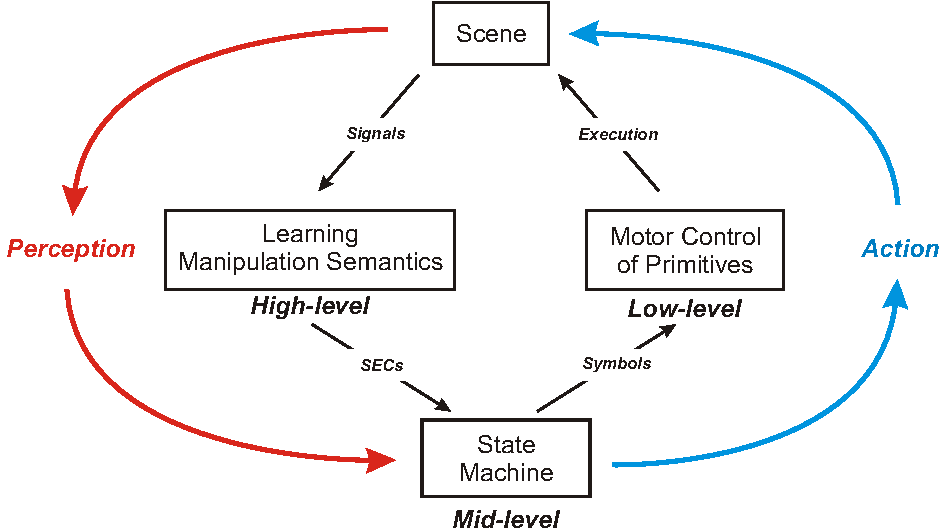
\includegraphics[scale=0.5]{./pdf/Figure_PerceptionAction.pdf}
      \caption{ Perception-action chain.}
      \label{fig:per_act_cycle}
\end{figure}

 
  

%\newpage  %% needed for single columns
\clearpage  %% needed for two columns
%%%%%%%%%%%%%%%%%%%%%%%%%%%%%%%%%%%%%%%%%%%%%%%%%%%%%%%%%%%%%%%%%%%%%%%%%%%%%%%%%%%%%%%%%%%%%%%%%%%%%%%%%%%%%
\section{State of the Art}
\label{sec:soa}

There exists a large corpus of work in action representation and execution \cite{Ijspeert2002,Ude93,Lee2006,Calinon2007}. Two distinct approaches are commonly preferred in order to represent and execute actions, one at the trajectory level \cite{Ijspeert2002} or the other at the symbolic level \cite{Dillmann2010}.
The former gives more flexibility for the definition of actions, while the latter defines actions at a higher level and allows for generalization and planning.

For trajectory level representation there are several well established techniques: splines \cite{Ude93}, Hidden Markov Models \cite{Lee2006}, Gaussian Mixture Models \cite{Calinon2007}, Dynamic Movement Primitives  \cite{Ijspeert2002,Luksch12}.
With trajectory level encoding, one investigates or learns different complicated trajectories, but it is difficult to use them in a ``more cognitive sense''. Generalization of the observed trajectories is the main {\it breaking~point} here, since even the same action can be demonstrated by following various trajectories.

High-level symbolic representations many times use graph structures and relational representations,
\eg \cite{Pardowitz2007,Ekvall2006,Aksoy2011}. Alternative methods, such as in \cite{Lee2013}, describe a syntactic approach for learning robot imitation by capturing  underlying task structures in the form of probabilistic activity grammars. 
These approaches give compact descriptions of complex tasks,
but they do not consider execution-relevant motion parameter (trajectories, poses, forces) in great detail.
In this work, our high-level action descriptor is based on the concept of Semantic Event Chains (SECs) introduced in  \cite{Aksoy2011}. 
SECs are generic action descriptors that capture the underlying spatiotemporal structure of continuous actions by sampling only
decisive key temporal points derived from the spatial interactions between hands and objects in the scene. The
SEC representation is invariant to large variations in trajectory, velocity, object type, and pose used in the action. 
Therefore, SECs can be employed for the classification task of actions as demonstrated in various experiments in  \cite{Aksoy2010,Aksoy2011,Aksoy2011b,Aksoy2013,AksoyRAS2014}. 
In contrast to works in  \cite{Pardowitz2007,Ekvall2006}, we have already shown in \cite{Aksoy2011b} that actions encoded by SEC can be executed once the low-level data (object positions, trajectories, etc.) are provided. 


  

The concept of semantic event chains has also  been successfully utilized and extended by others \cite{Waechter2013,Luo2011,Vuga2014,David2014} for monitoring or execution purposes. The work in \cite{Waechter2013} addressed the reproduction of the obtained human action sequence by parameterizing semantic conclusive sub-actions with the SEC framework.
Active learning of goal directed manipulation sequences, each was recognized using semantic similarities between event chains, was presented in \cite{David2014}. Scene graphs used in SECs were also represented with kernels in \cite{Luo2011} to further apply different machine learning approaches. Additional trajectory information was used in \cite{Vuga2014} to reduce noisy events occur in SECs. All these studies confirm the scalability of the event chains to various monitoring tasks.

Many times trajectory-level descriptions of actions, object properties, and high-level goals of the manipulation are brought together through STRIPS-like planning \cite{Dillmann2010}, resulting in operational although not very transparent systems. The approach in \cite{Ahmadzadeh2015} attempts to integrate symbolic action 
representation and planner with motor skill learner. The robot learns the goal of the human demonstrated actions by using
the Visuospatial Skill Learning (VSL) method which produces symbolic predicates. Such predicates are directly fed to a standard planner to encode skills in a discrete symbolic form. The proposed framework also considers the sensorimotor skills, such as the followed trajectory information from
the observed action. 
In contrast to the work in  \cite{Ahmadzadeh2015}, we do not require additional symbolic planner since SECs provide an observable state sequence which substitutes the symbolic planner. Such approaches are also not evaluated on long and complex human manipulation actions. 
Thus, how to bring these trajectory and  symbolic levels together remains a big challenge in robotics.

\red{SoA section needs to be extended to, at least, one page!...}


\clearpage  %% needed for two columns

 








%%%%%%%%%%%%%%%%%%%%%%%%%%%%%%%%%%%%%%%%%%%%%%%%%%%%%%%%%%%%%%%%%%%%%%%%%%%%%%%%%%%%%%%%%%%%%%%%%%%%%%%%%%%%%
\section{Method}
\label{sec:method}

As illustrated in Fig.~\ref{fig:per_act_cycle} our proposed perception action framework involves three main levels: {\it high-}, {\it mid-}, and {\it low-level} action units. In this section we will provide the detailed description of each level together with their components as depicted in the block diagram in Fig.~\ref{fig:blockdiagram}.
  
  
 \begin{figure}[!t]
      \centering
      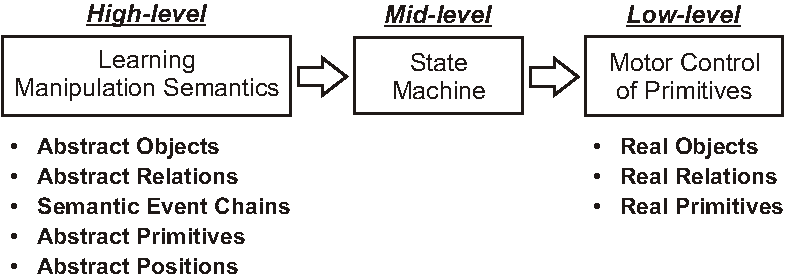
\includegraphics[scale=0.62]{./pdf/Figure_BlockDiagram.pdf}
      \caption{ Block diagram of the algorithm.}
      \label{fig:blockdiagram}
\end{figure}

 

%%%%%%%%%%%%%%%%%%%%%%%%%%%%%%%%%%%%%%%%%%%%%%%%%%%%%%%%%%%%%%%%%%%%%%%%%%%%%%%%%%%%%%%%%%%%%%%%%%%%%%%%%%%%%
\subsection{High-level Action Definition}
\label{sec:high-level}

In this first section we will give a high-level definition of manipulation actions. Note that at this level, definitions are mainly symbolic, abstract, and close to human description.


Take an example of a manipulation action   {\it ``putting a bucket on a box''} in which a hand is putting a bucket on top of a box.  Fig.\ref{fig:put_on_action} shows some sample frames from a human demonstration.
This simple action may be described by a human as follows:

\begin{enumerate}
  \item \textbf{\textit{Approaching}} to the bucket,
  \item \textbf{\textit{Grasping}} the bucket,
  \item \textbf{\textit{Putting}} the bucket on the box, and
  \item \textbf{\textit{Releasing}} the bucket.
\end{enumerate}

This description is by no means unique.
One could easily describe the same action in different words, with different number of steps and  details.
However, one could still extract some common and descriptive properties from such a naive description:

\begin{itemize}
  \item[$\bullet$] \textbf{Property 1:} The definition is still valid even if the objects are altered.
  \item[$\bullet$] \textbf{Property 2:} An action can be broken into a sequence of smaller primitives such as \textit{approach} and \textit{grasp}.
  \item[$\bullet$] \textbf{Property 3:} There are conditions to end one primitive and start the next. In the above example these conditions are rather implicit.
  \item[$\bullet$] \textbf{Property 4:} As humans, we intuitively know how to  perform these primitives, although our exact movements are produced when we see the objects and perform the action.
\end{itemize}


Our approach to execute human-like actions with robots is similar to this simple example.
We introduce a generic high-level definition of actions which is independent from the manipulated objects in the action ({\it Property 1}),
and consists of a sequence of primitives ({\it Property 2}).
The conditions to start and end each primitive are defined %explicitly ({\it Property 3}).
implicitly by considering the contact relation between the hand and  objects in the action ({\it Property 3}).
We also store the default trajectory parameters to execute actions in the high-level definition.
When novel real objects are observed at each specific instance of an action, these parameters are employed to generate the required movements ({\it Property 4}).

 
\begin{figure*}[!hb]
  \centering
    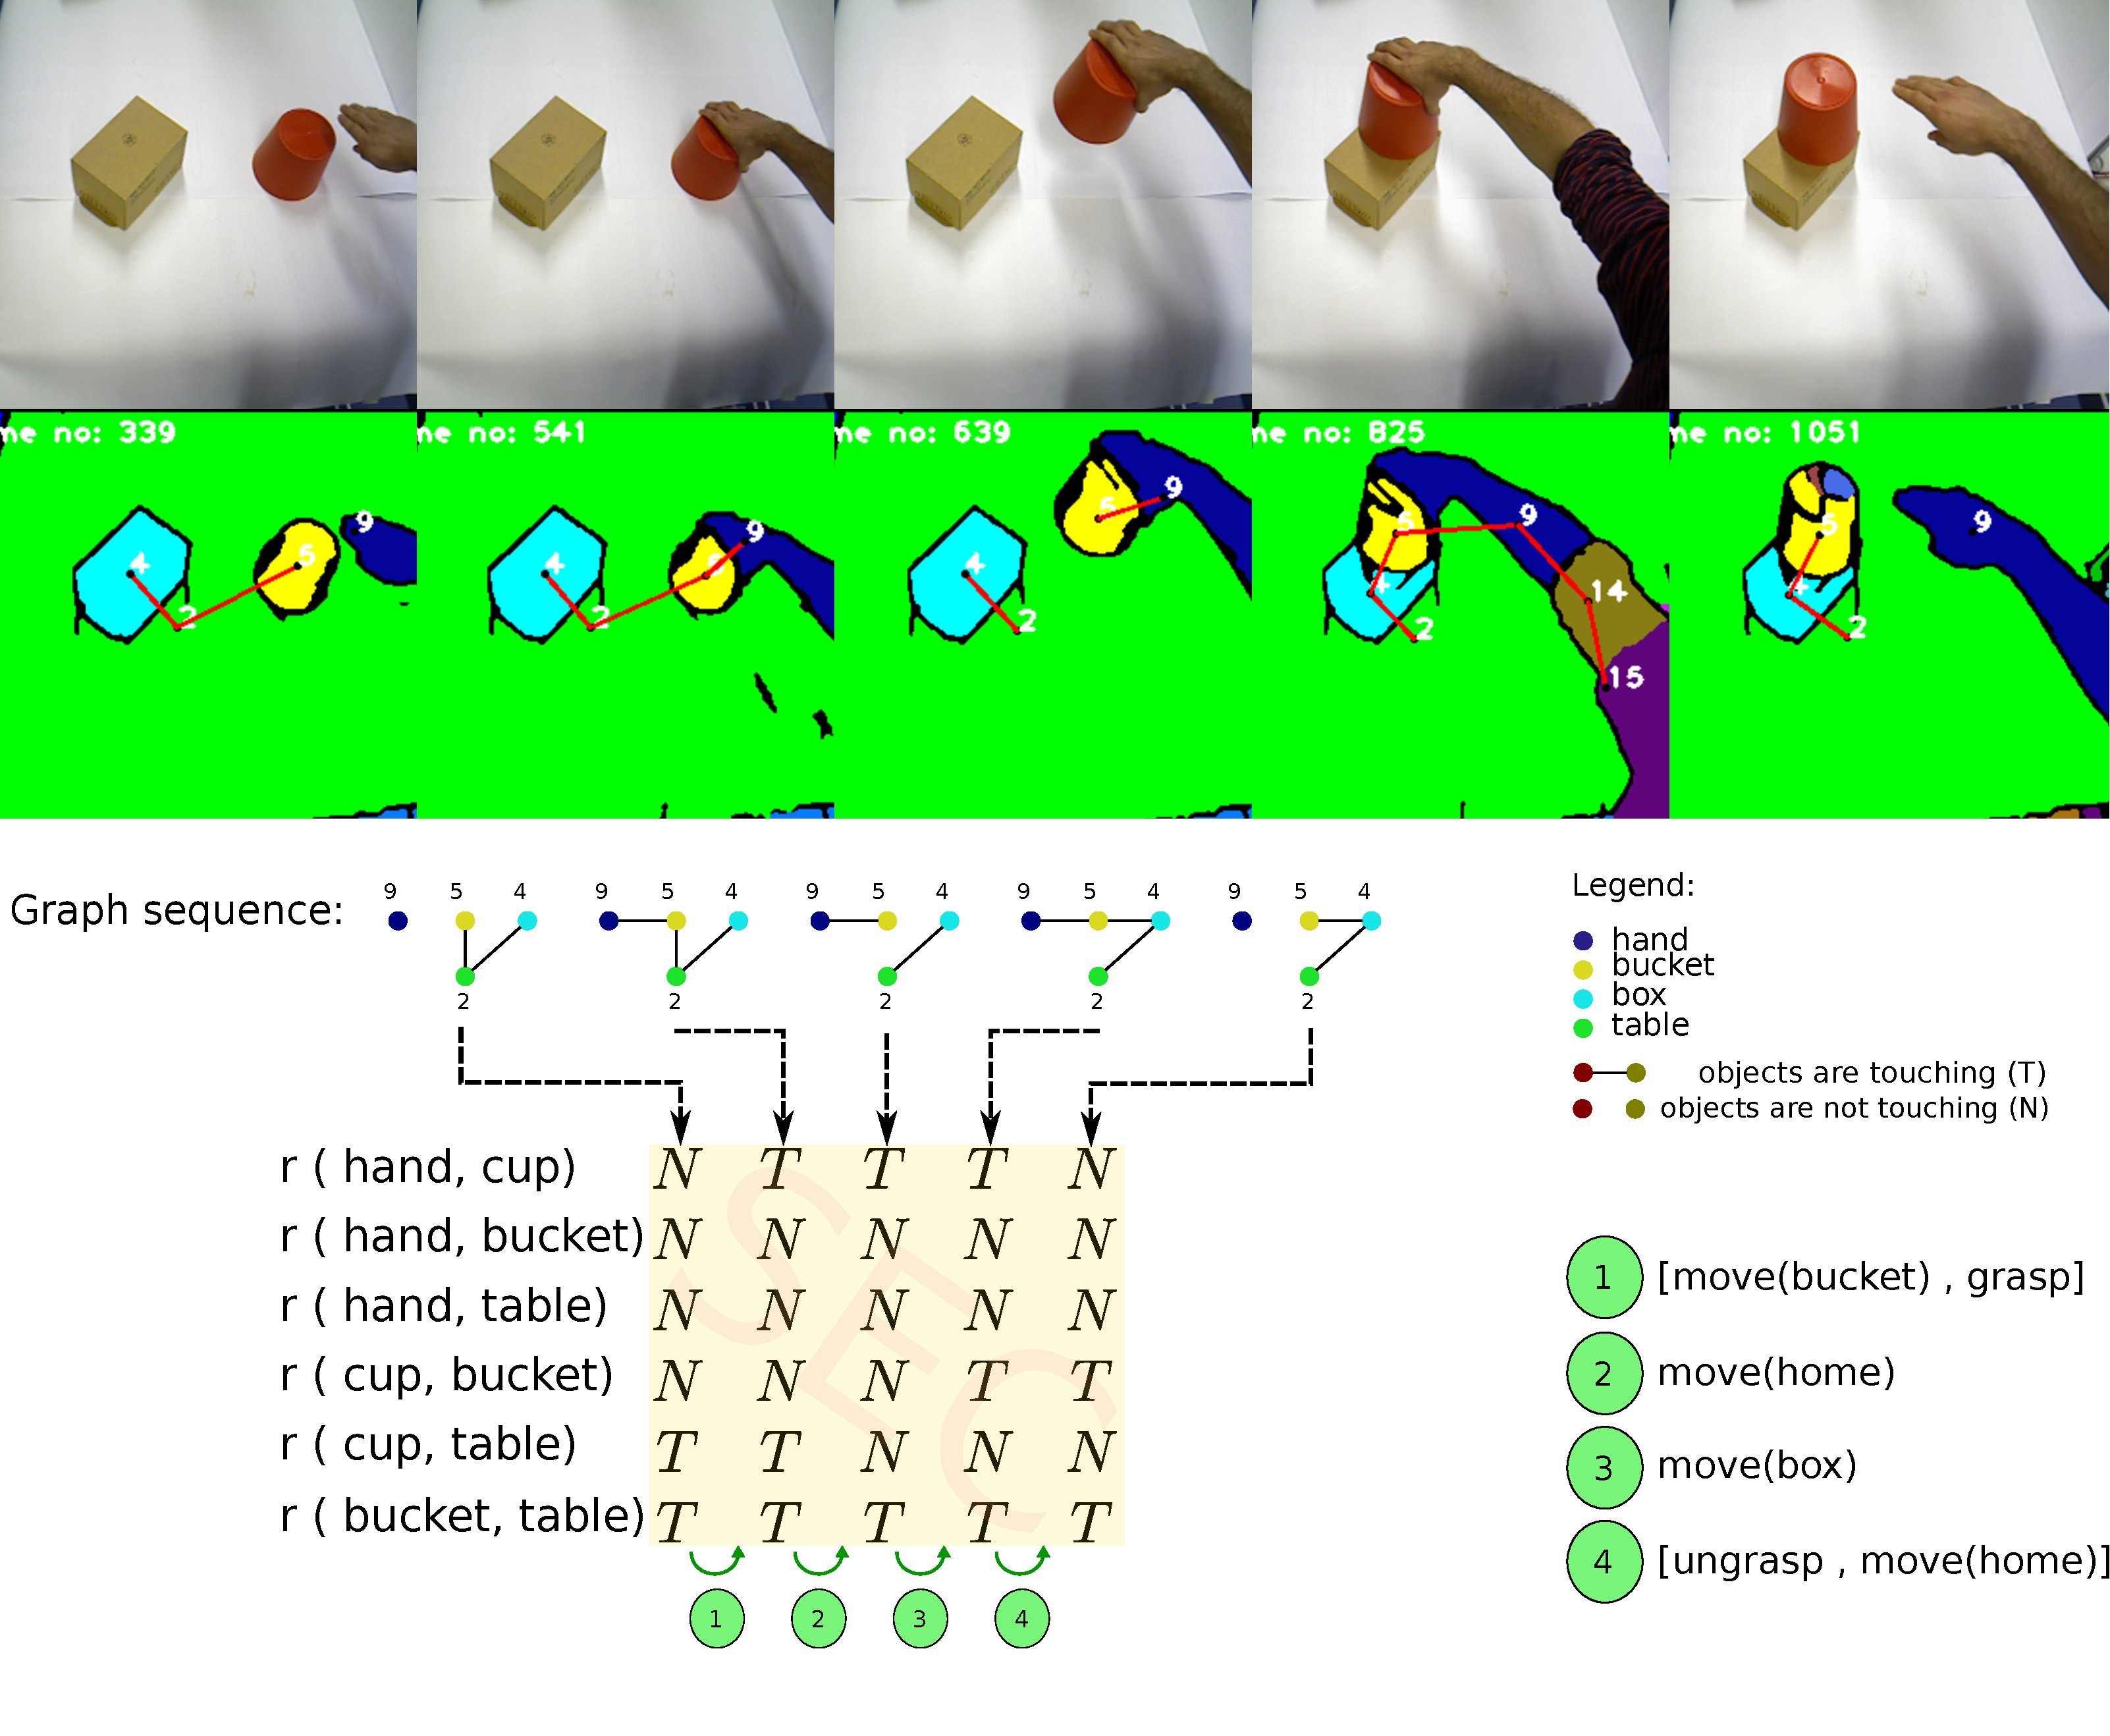
\includegraphics[scale=0.25]{./pdf/action_graph_sec.pdf}
      \caption{ SEC representation of a human demonstrated {\it ``putting a bucket on a box''} action.      
       The snapshots of the performed action together with segmented images are shown on the top. 
       The symbolic graph sequence is given in the middle. Each graph corresponds to one column in the SEC matrix given in the bottom left. Corresponding action primitives are shown on the bottom right.
Abstract objects are the {\it  manipulator}, {\it primary object}, {\it secondary object}, and {\it background}.  Real objects are the {\it hand}, {\it  bucket}, {\it  box} and {\it  table}, respectively.}
      \label{fig:put_on_action}
\end{figure*}

 
To fully satisfy these four properties in our high-level action definition, we benefit from the  \textit{ontology of manipulation actions} introduced in \cite{TAMD13}.
This ontology structures human demonstrated manipulation actions, \eg~{\it putting a bucket on a box}, as sequences of spatiotemporal interactions between objects and hands in the scene by using the concept of Semantic Event Chains (SECs) presented in \cite{Aksoy2011}. 
The hypothesis claims that the most important information are encoded at the decisive temporal anchor points, \ie when touching relations between objects and hands change. Considering this claim, the ontology suggests $30$ fundamental and unique manipulations that allow complex and chained activities, \eg {\it ``making salad''} or {\it ``preparing breakfast''}.

The ontology introduces $4$ essential constraints on the definition of manipulation actions, which are stated as the following action descriptive rules: 


\begin{itemize}
 \item[$\bullet$] \textbf{Rule 1:} The action is performed by one hand. This is true for the most of human actions, since the second hand is usually used as support.
 \item[$\bullet$] \textbf{Rule 2:} The hand touches at most one object in the course of action and does not purposefully touch another object in the scene unless the current action ends.
 \item[$\bullet$] \textbf{Rule 3:} The hand is free at the beginning and at the end of the action.
 \item[$\bullet$] \textbf{Rule 4:} The action must lead to some changes in the touching relations between objects and hands (\eg human or robot hand).
\end{itemize}



The first two rules in the ontology suggest that there is only one hand and at most one object that plays a specific role with the hand. We will describe in section~\ref{sec:abstractobjects} that actions can be isolated from object types  as required in {\it Property 1} by only considering roles of manipulated objects. The second rule is also introduced to make sure that the defined actions cannot be further split into shorter actions, which fulfills {\it Property 2}. The third  rule defines the natural start and end points of the manipulation for {\it Property 3}. The last rule assures that hands and manipulated objects are the only ones having direct interaction with each other and consequently affecting the dynamics of the manipulation. Parameters of these interactions are the required elements in {\it Property 4} to reproduce the action. In the rest of this section, we will describe several components in our high-level symbolic action definition that are required to reach these descriptive properties.
We refer the interested reader to \cite{TAMD13} for details of the manipulation action ontology. 





%%%%%%%%%%%%%%%%%%%%%%%%%%%%%%%%%%%%%%%%%%%%%%%%%%%%%%%%%%%%%%%%%%%%%%%%%%%%%%%%%%%%%%%%%%%%%%%%%%%%%%%%%%%%%
\subsubsection{Abstract Objects}
\label{sec:abstractobjects}

There present many  objects in the real-world scenes.
It is thus not practical to define a separate action for each possible object.
Instead, as stated in {\it Property 1}  in section~\ref{sec:high-level}, we represent manipulation actions in a generic way to make them applicable to any novel object.
In this regard, we label objects by their roles exhibited in the action. In other words, objects are abstracted to their roles in the action.
First of all, recalling {\it Rule 1} in the ontology given in section~\ref{sec:high-level}, we assume that one actor is needed that performs the main goal in the action, which is here called \textit{manipulator}. As stated in {\it Rule 2}, there exists at most one object that is manipulated directly by the manipulator.
This object is called \textit{primary object}. All other objects, which are interacted with the primary object, are called {\it secondary objects}.
For example, in the action {\it ``putting a bucket on a box''}  depicted in Fig.\ref{fig:put_on_action}, the human hand is the \textit{manipulator}, the bucket which is directly manipulated by the hand is the \textit{primary object}, and the box is the only {\it secondary object} as it is interacting with the primary object, \ie bucket.
Note that for the sake of simplicity we assume that there exist only one {\it secondary object} in the action. 
%Note that unlike \textit{primary objects}, there could be multiple {\it secondary objects} in an action as will be shown in  chained actions in  section~\ref{sec:results}.  

Additionally, we treat the supporting plane, \ie~{\it background}, as another object that affects the fate of the action. The main advantage coming with the {\it background} is the term ``air-phase'' in actions, 
which emerges when the \textit{primary object} is lifted and moving in the air, but it is not yet touching any other object, \eg~{\it background} or \textit{secondary object}. Therefore, this term allows the robot to seamlessly execute the primitives such as {\it lift} or {\it place}.

Consequently, the number of abstract objects in our high-level action definition is at most four: \textit{manipulator}, \textit{primary object}, \textit{secondary object}, and {\it background}.
 



\begin{table*}[!hb]
\centering
\caption{Abstract relations and their attributes for the action {\it ``putting a bucket on a box''} shown in Fig.\ref{fig:put_on_action}.}
\begin{tabular}{ lllll }
\hline\noalign{\smallskip}
Relation Name & Abstract Relation & Real Relation & Type \\
\noalign{\smallskip}\hline\noalign{\smallskip}
$\text{R}_1$  & R(manipulator,primary object) & R(hand,bucket) & variable \\
$\text{R}_2$  & R(manipulator,secondary object)& R(hand,box) & don't-care \\
$\text{R}_3$  & R(manipulator,background) & R(hand,table) & don't-care \\
$\text{R}_4$  & R(primary object,secondary object) & R(bucket,box) & variable  \\
$\text{R}_5$  & R(primary object,background) & R(bucket,table) & variable \\
$\text{R}_6$  & R(secondary object,background)& R(box,table) & constant \\
\noalign{\smallskip}\hline
\end{tabular}
\label{tab:relations}
\end{table*}



%%%%%%%%%%%%%%%%%%%%%%%%%%%%%%%%%%%%%%%%%%%%%%%%%%%%%%%%%%%%%%%%%%%%%%%%%%%%%%%%%%%%%%%%%%%%%%%%%%%%%%%%%%%%%
\subsubsection{Abstract Relations}

Once the abstract objects in the action are extracted, we continue with computing the spatial relations between each objects pair, \eg between the {\it manipulator} and the {\it primary object}.
If there exists $n$ objects in an action, the number of distinct relations is given by  $n(n-1)/2$.
As stated before, there are $4$ abstract objects in our high-level action definition, which yields in total 6 abstract relations. Table \ref{tab:relations} shows all possible abstract relations for the scenario {\it ``putting a bucket on a box''} depicted in Fig.\ref{fig:put_on_action}.


Each relation is defined by two attributes, namely 	\emph{type} and \emph{value}.
The \emph{type} of a relation is determined by the importance and variation of that relation throughout the action.
For example, for the same action in Fig.\ref{fig:put_on_action}, the relation between the {\it manipulator} and the {\it background} does not affect the outcome of the action. Therefore, the type of such relations is \emph{don't-care}. Although the importance of some relations is decided based on a common sense, many of them were learned during the observation phase as addressed in \citep{AksoyRAS2014}.

Other relations, which are crucial for an action, are categorized as \emph{variable} and \emph{constant} relations.
For example, the relation between the {\it manipulator} (\ie hand) and {\it primary object} (\ie bucket) in Fig.\ref{fig:put_on_action} is \emph{variable} since it alters during the action. On the other hand,
the relation between the  {\it secondary object} (\ie box) and the  {\it background} (\ie table) remains the same and hence is \emph{constant}.
We note that such constant relations highlight the necessary pre-conditions to perform an action and any change in these constant relations implies failure of the action.
On the other hand, variable relations encode the progress of the action and play the most important role in our methodology.

Possible  \emph{values} of an abstract spatial relation are {\it Not touching} ($N$), {\it Touching} ($T$), and {\it Absence} ($A$), where $N$ corresponds to two spatially separated objects, $T$ represents objects that touch each other.  The  value $A$ occurs when there exists no information about the relation, \eg one object is not defined or not visible.
 


%%%%%%%%%%%%%%%%%%%%%%%%%%%%%%%%%%%%%%%%%%%%%%%%%%%%%%%%%%%%%%%%%%%%%%%%%%%%%%%%%%%%%%%%%%%%%%%%%%%%%%%%%%%%%
\subsubsection{Semantic Event Chain (SEC)}
\label{sec:SEC}

Actions in the ontology (see section~\ref{sec:high-level}) are encoded by  the concept of the Semantic Event Chains (SECs) introduced in \cite{Aksoy2011}. 
SECs capture the essence of an action by employing computer vision techniques. Image sequence of an observed action is first represented by image segments each of which corresponds to one object in the scene and is consistently tracked during the action. Each frame in the sequence is then converted into a graph: nodes represent tracked segments, \ie objects, and edges indicate the touching relation between a pair of objects.  	
By employing an exact graph matching method, the continuous graph sequence is discretized into decisive main graphs, \ie ``states", each of which represents a topological change in the scene. 
All extracted main graphs form the core skeleton of the SEC, which is a matrix where rows are the abstract spatial relations (\eg touching) between object pairs.
Each column of SEC matrix is interpreted as a state of the scene, which is a combination of the relations between the objects when a new main graph occurs. 


As there are six abstract relations in our high-level action description, the SEC matrix has always $6$ rows.
On the other hand, the number of SEC columns depends on how many times the relations between objects change in the course of action and hence can alter from action to action.

The valid symbolic entries in the SEC matrix are the abstract relations, \ie N (Not touching), T (Touching) and A (Absence). In a SEC, the progress of the action from the beginning to the end, is seen in a compact way.
In addition, the SEC matrix is invariant to large variations in trajectory, velocity, object type, and pose used in the action and therefore remains the same for different instances of one action.
Fig.\ref{fig:put_on_action} shows the extracted final SEC matrix together with corresponding main graphs, \ie states, and respective tracked segments (colored regions) for the the scenario {\it ``putting a bucket on a box''}.



\clearpage  %% needed for two columns
%%%%%%%%%%%%%%%%%%%%%%%%%%%%%%%%%%%%%%%%%%%%%%%%%%%%%%%%%%%%%%%%%%%%%%%%%%%%%%%%%%%%%%%%%%%%%%%%%%%%%%%%%%%%%
\subsubsection{Abstract Primitives}
\label{sec:abstract_primitives}
In the simple example at the beginning of this section, it is shown that a full action can be divided into several primitives.
These primitives or \textit{primitives} are the basic functions of the manipulator.

In our approach we define the following primitives:
\begin{itemize}
 \item $move(pose)$ :  The manipulator moves to $pose$.
 \item $move_{periodic}(path)$ : The robot arm moves periodically along the given path.
 \item $force()$ : The robot arm exerts $force$.
 \item $grasp()$ : The robot hand grasps an object.
 \item $release()$ : The robot hand releases an object.
\end{itemize}


These primitives are the basic functions of our hardware which can be implemented in many different ways.
The focus of our work is not implementing these primitives,
but rather we would like to propose a way to combine them to produce actions.
Nevertheless, our implementations are presented in section.\ref{section_primitives}.

In Fig.\ref{fig:put_on_action}, the necessary primitives associated to each column of the SEC matrix are shown.
There number of primitives at each phase is either one or two.
The reason to add a second primitive is that sometimes more than one primitives are needed to make the desired event \ie the desired change in the relations.
For example, a combination of $move(pose)$ and $grasp()$ primitives are often necessary to grasp an object.

xxx here, each state transition from one column (state) to the next defines one unique primitive.


%%%%%%%%%%%%%%%%%%%%%%%%%%%%%%%%%%%%%%%%%%%%%%%%%%%%%%%%%%%%%%%%%%%%%%%%%%%%%%%%%%%%%%%%%%%%%%%%%%%%%%%%%%%%%
\subsubsection{Abstract Positions}

As described above, one important primitive is the $move(pose)$ primitive that moves the robot arm toward a pose.
In the abstract definition, the argument $pose$ of this primitive is an abstract position.
The abstract positions are either the objects in the scene, or some other convenient points in space.
While performing the actions, sometimes we move our hands toward points in space where exist no specific objects.
One example is when we initially lift an object from a table, to put it on top of another object.
We move the object to a point that makes our next move easier.
We call such positions \textit{home}.

In some actions, we need to move toward arbitrary positions to achieve the goal of the action.
For example in the pushing action, we push an object to a desired position.
This desired position could be any accessible point and it is usually specified by the user or a higher level planner.
We call this type of abstract positions the \textit{goal} position.



%%%%%%%%%%%%%%%%%%%%%%%%%%%%%%%%%%%%%%%%%%%%%%%%%%%%%%%%%%%%%%%%%%%%%%%%%%%%%%%%%%%%%%%%%%%%%%%%%%%%%%%%%%%%%
\subsection{Low-level Action Definition}
\label{sec:low-level}
In this section, the abstract components of the high-level definition are related to their real-world counterparts.
This includes defining objects in the real world, implementing the low-level primitives such that proper commands are sent to the hardware control systems,
and calculating the object relations from the sensor data.
In the rest of this section, these steps are described in more detail.


%%%%%%%%%%%%%%%%%%%%%%%%%%%%%%%%%%%%%%%%%%%%%%%%%%%%%%%%%%%%%%%%%%%%%%%%%%%%%%%%%%%%%%%%%%%%%%%%%%%%%%%%%%%%%
\subsubsection{Real objects}
In the real world experiments, the abstract objects (\textit{manipulator}, \textit{primary object}, \textit{secondary object}, and \textit{background})
are instantiated by real objects in the scene.
For the put-on-top example depicted in Fig. \ref{fig:put_on_action},
these objects are manipulator=hand, primary object=bucket, secondary object=box, and background=table.
We need to represent the real-world objects in the signal space so that we can perform the primitives.

In our work, two pieces of information is needed to represent an object.
First, the position of each object with respect to some fixed frame is needed.
Note that the frame is fixed to the workspace of the robot.
To associate a position to the object, the objects are modeled with a single point, located at their center of mass.
Second, the direction of objects in the XY-plane should be detected.
This is necessary for grasping the objects, as well as some actions like cutting.
Note that we use this direction information only for elongated objects (such as cucumber) but not for symmetric objects (such as apple, cup etc.)
The direction is defined as the angle that the main axis of the object makes with respect to the X-axis of the reference frame.

To this end, we use our vision system to represent each object in the scene with a point cloud.
\textcolor{red}{Eren: a short description of vision system is needed}
Using the point cloud we can calculate the center of mass of the object.
To calculate the direction of the objects, we use principle component analysis (PCA) to find the major axis of the object.
The direction of the object is defined as the direction of its major axis.

\begin{table*}
\centering
\caption{Summary of object relation detection in different actions. For each relation only the main sensor is mentioned.}
\begin{tabular}{ lcccccc }
\hline\noalign{\smallskip}
 Action Name &  $\text{R}_1$ & $\text{R}_2$ &$\text{R}_3$ &$\text{R}_4$ &$\text{R}_5$&$\text{R}_6$ \\
\noalign{\smallskip}\hline\noalign{\smallskip}
 Pick and Place & tactile & -       & position & -     &  force & - \\
 Put-on-top     & tactile & tactile & position & force &  vision & vision \\
 Take-down      & tactile & tactile & position & vision&  force & vision \\
 Put-in         & tactile & tactile & position & force &  vision & vision \\
 Cut            & tactile & tactile & position & force &  position & vision \\
 Unload         & tactile & tactile & position & vision&  force & vision \\
 Stir           & tactile & -       & position & vision&  vision & - \\
 Push           & force   & -       & position & -     &  vision & - \\
 Poke           & force   & -       & position & -     &  vision & - \\
\noalign{\smallskip}\hline
\end{tabular}
\label{tab:relation_detection}
\end{table*}



%%%%%%%%%%%%%%%%%%%%%%%%%%%%%%%%%%%%%%%%%%%%%%%%%%%%%%%%%%%%%%%%%%%%%%%%%%%%%%%%%%%%%%%%%%%%%%%%%%%%%%%%%%%%%
\subsubsection{Real relations}
\label{sec:real_relations}
The real relations are the actual relations between pairs of objects.
These relations together form a symbolic representation of the scene, or in other words, the current state of system.
To detect the relations, we use combination of vision, position, force, and tactile sensors.

When it comes to detecting the object relations, there are three distinct phases: before the action, during the action, and after the action.
In the first and last phases, the main source of information is the vision system.
In the middle phase , when the action is being performed, the sensors of the robot play the main role,
and the vision system acts as a support to confirm the outcome of these sensors.

At the beginning and the end of the action, we have some objects located on a background, and a manipulator which is away from the objects.
This is a result of the Rule.3 (see Section.\ref{sec:high-level}) in the ontology.
This requires the first three relations (the relation of manipulator with the objects and the background) to be equal to N.
The vision system can detect that we are in a proper state.
The tactile sensors of the robot hand are also used to confirm that no object is grasped by the hand.
The last three relations can only be detected by vision.
These are the relations of the primary object, the secondary object, and the background.

During the action, the relations of the objects are calculated by combining data from different sensors.
The sensors used for each relation and how the data from different sensors are combined, depends on the type of the action.
Next we describe how these relations are calculated in the put-on-top action.

The relation of the manipulator with the primary and secondary objects are calculated from the position and tactile sensors.
When the position of the manipulator is close to the \textit{primary} (\textit{secondary}) object and the tactile sensors sense that the manipulator has grasped something,
$\text{R}_1$ ($\text{R}_2$), is switched to T.
Although we can detect the $\text{R}_2$, usually this relation is not important and marked as don't-care.
The reason is that the manipulator does not directly interact with the secondary object.

The relation of the manipulator and the background ($\text{R}_3$) plays no important role in this action, so we label it as don't-care.
This is not specific to this action and for all other actions the $\text{R}_3$ is don't-care.


The relation of the primary object and the secondary object ($\text{R}_4$) is calculated by force sensor of the robot arm.
However, this depends also on the relation of manipulator and primary object, and on the position sensor.
In short, when the manipulator holds the primary object and it approaches the secondary object,
if the force sensor reads a contact force in the opposite direction of movement, the relation is changed to touching (T).
The position sensor is used to confirm that the relative pose of the objects is correct and they are close enough for a contact.
The relation of primary object and the background ($\text{R}_5$) is also detected in a similar way.

The relation of the secondary object and the background ($\text{R}_6$) is a constant relation and is detected by vision.
For the cases that other sensors than vision are used, the vision sensor is also employed to confirm the resulting event.
The sensors used to detect relations during different actions are summarized in table.\ref{tab:relation_detection}.


%%%%%%%%%%%%%%%%%%%%%%%%%%%%%%%%%%%%%%%%%%%%%%%%%%%%%%%%%%%%%%%%%%%%%%%%%%%%%%%%%%%%%%%%%%%%%%%%%%%%%%%%%%%%%
\subsubsection{Low-level primitives}
\label{section_primitives}
In section.\ref{sec:abstract_primitives} we defined the primitives which are performed by the manipulator.
Here we describe our implementation of these primitives at the low-level.

For the robot arm, we have three primitives: $move(p_{des},P)$, $move_{periodic}(W)$, and $exert(F)$.
The first two primitives generate trajectories for the position control of the robot.
To generate the trajectories in the Cartesian space, we use dynamic movement primitives (DMP) with joining introduced in \cite{Kulvicius2012}.
The argument $P$ represents the parameters of the DMP which consist of parameters of Gaussian kernels and the time of trajectory $T$.
The parameters of the kernels are the number $n$, width $\sigma$, and weights $W$.
The details of implementation are not covered here \red{cite some papers here!}, but the final result is that by using the primitive $move(p_{des},P)$
we can move the robot arm from the current position and orientation, to any desired position and orientation, along the desired trajectory.

The $exert(f_{des},P)$ performs force control with set-point $f_{des}$.
In our setup, we use a parallel force/position scheme with dominant force control, similar to \cite{chiaverini1993parallel}.
In this way we can achieve the desired force in the constrained space, and at the same time, perform desired motions in the unconstrained space,
the trajectory of which is defined by $P$.


To grasp objects we use velocity control of finger joints together with feedback from tactile sensors on the fingers.
We use separate pre-shapes for round and elongated objects.
This provides grasps for simple objects, which is enough to demonstrate our system.
The complex problem of grasping arbitrary objects is not a goal of this research.

XXX mention that we have two grasp types: power and precision


%%%%%%%%%%%%%%%%%%%%%%%%%%%%%%%%%%%%%%%%%%%%%%%%%%%%%%%%%%%%%%%%%%%%%%%%%%%%%%%%%%%%%%%%%%%%%%%%%%%%%%%%%%%%%
\section{Implementing the Actions}
\label{sec:Implementing}

In this section we present our implementation of manipulation actions based on the high-level and low-level definitions given in the previous sections.
First we introduce the hardware setup used in the experiments.
Then, we present the software components that are developed as part of the library of actions.
Finally, our algorithm for executing actions is described as a finite state machine.



%%%%%%%%%%%%%%%%%%%%%%%%%%%%%%%%%%%%%%%%%%%%%%%%%%%%%%%%%%%%%%%%%%%%%%%%%%%%%%%%%%%%%%%%%%%%%%%%%%%%%%%%%%%%%
\subsection{Hardware}
\label{sec:hardware}
The action library is designed to execute actions on a general robotic arm/hand system.
Here we describe the hardware in our setup as used in the experiments in section \ref{sec:results}.
Our setup consists of a 7-DOF KUKA LWR robot manipulator, a three-fingered robotic hand and a vision system. 
The vision system is a RGB-D camera. \textcolor{red}{Eren: please rewrite this sentence if necessary.}


%%%%%%%%%%%%%%%%%%%%%%%%%%%%%%%%%%%%%%%%%%%%%%%%%%%%%%%%%%%%%%%%%%%%%%%%%%%%%%%%%%%%%%%%%%%%%%%%%%%%%%%%%%%%%
\subsubsection{Robot Arm}
Our robot arm is a KUKA LWR (Light Weight Robot) IV manipulator.
It is a kinematically redundant anthropomorphic manipulator developed jointly by KUKA Robot Group and the German Aerospace Center (DLR).
It has 7 DOFs and is equipped with position and torque sensors at each joint.
It estimates the external torques applied to each joint which also gives an estimate of external force and torque at the end effector.
The robot can be commanded both in joint space and Cartesian space, with variable compliance and damping.

By using a C++ library called the Fast Research Interface (FRI) it is possible to communicate to LWR's control system and sensors, from an external PC.


%%%%%%%%%%%%%%%%%%%%%%%%%%%%%%%%%%%%%%%%%%%%%%%%%%%%%%%%%%%%%%%%%%%%%%%%%%%%%%%%%%%%%%%%%%%%%%%%%%%%%%%%%%%%%
\subsubsection{Robot Hand}
Our robot hand is a SDH-2 (Schunk Dexterous Hand 2) produced by the Schunk company.
It has three fingers and 7 degrees of freedom, which can be controlled in position or velocity modes.
It has tactile sensors that provide feedback when grasping objects.


%%%%%%%%%%%%%%%%%%%%%%%%%%%%%%%%%%%%%%%%%%%%%%%%%%%%%%%%%%%%%%%%%%%%%%%%%%%%%%%%%%%%%%%%%%%%%%%%%%%%%%%%%%%%%
\subsubsection{Vision System}
Our vision system includes an RGB-D camera (Microsoft Kinect) and a DSLR camera.
\textcolor{red}{Eren: please develop this part}


%%%%%%%%%%%%%%%%%%%%%%%%%%%%%%%%%%%%%%%%%%%%%%%%%%%%%%%%%%%%%%%%%%%%%%%%%%%%%%%%%%%%%%%%%%%%%%%%%%%%%%%%%%%%%
\subsection{Software}
\label{sec:software}
The library of actions is implemented as an application in the Open Robot Control Software (Orocos) framework \cite{rtt-url,soetens2006}.
The Orocos is a framework to develop real-time robotic and automation applications.
In a typical Orocos application, several components exist which communicate over (possibly real-time) data ports.
The library of actions consists of several components which are shown in fig.\ref{fig:software_structure}.
Some of the components communicate to hardware (Sensors and actuators), while others perform calculations and control the execution of actions.
The components are described in the following:
\begin{figure*}
      \centering
      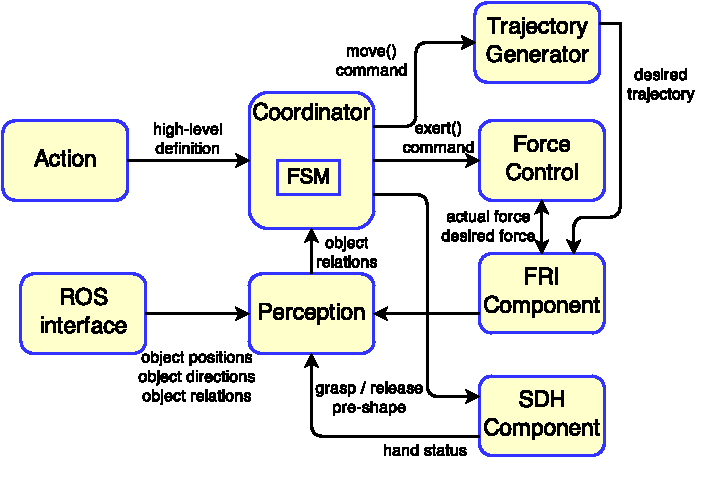
\includegraphics[scale=1]{./pdf/software_structure.pdf}
      \caption{ Block diagram of the software for action library.
      The interconnection of the components are shown as well as the interface to ROS nodes and hardware.
      \red{needs to be updated!...}
}
      \label{fig:software_structure}
\end{figure*}



\begin{itemize}
 \item{\textbf{Action}}
component holds the parameters of the high-level definition of the action.
These parameters are the SEC matrix, high-level primitives, and the abstract arguments.
The parameters of the DMP for trajectories are also stored in this component.
\item{\textbf{Perception}}
component collects data from all the sensors and determines if the relations of objects in the scene are altered.
It receives the object poses from the vision system (through the ROS-interface component).
It also monitors other sensors and detects changes in object relations according to section.\ref{sec:real_relations}.
\item{\textbf{Coordinator}}
component contains a state machine that executes the action.
The detail of the state machine and execution algorithm will be discussed in \ref{sec:execution_algorithm}.
Additionally, some function like comparing desired and actual relations is done inside this component.

\item{\textbf{Trajectory Generator}}
component receives $move()$ and $move_{periodic}()$ primitives and generates the trajectory using the DMPs.

\item{\textbf{Force Control}}
component implements the $exert()$ primitive.
The actual contact force is received from the FRI component and using the algorithm of section.\ref{section_primitives},
the contact force is regulated in the desired direction.
The output of this component is sent to the control system of the LWR arm, though the FRI component.

\item{\textbf{FRI}}
component communicates with the robot arm through the FRI,
and provides the necessary input and output data ports to other Orocos components.

\item{\textbf{SDH}}
component implements the hand primitives (grasp, release, and pre-shape).
This component uses the C++ library which is provided to communicate with the Schunk SDH-2 robot hand.
The tactile sensor data are also processed in this component to detect objects in the hand.
The parameter $hand\_status$ determines the current status of the hand and is sent to the perception component.
This parameter takes values: Undefined, Grasped, and Empty

\item{\textbf{ROS interface}}
component creates an interface between the ROS nodes and Orocos data ports.
The data ports in Orocos are capable of talking to ROS nodes, using the components of $rtt\_ros\_integration$ stack.
% \footnote{http://wiki.ros.org/rtt_ros_integration}.
This component is created using the $rtt\_rosnode$ component of this stack to integrate all ROS communications in one component.
Since our vision system is developed in ROS framework, this component is used to get the information such as 
objects poses and relations from the vision system and create the necessary data ports to send them to other components.
\end{itemize}



\begin{figure*}
      \centering
      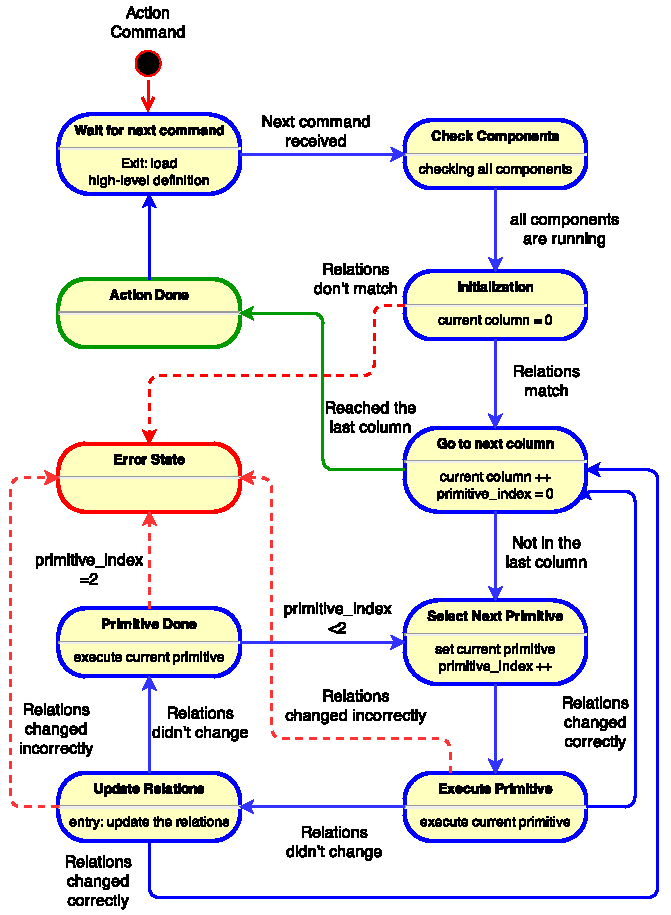
\includegraphics[scale=1]{./pdf/coordinator_fsm.pdf}
      \caption{ State diagram of the finite state machine governing the execution of action.
}
      \label{fig:coordinator_fsm}
\end{figure*}


%%%%%%%%%%%%%%%%%%%%%%%%%%%%%%%%%%%%%%%%%%%%%%%%%%%%%%%%%%%%%%%%%%%%%%%%%%%%%%%%%%%%%%%%%%%%%%%%%%%%%%%%%%%%%
\subsection{Execution Algorithm}
\label{sec:execution_algorithm}

Here an algorithm is presented to execute actions, using the software components introduced earlier.
The core of the execution is a finite state machine inside the coordinator component.

To implement the state machine, we use the $State\_Machine$ class in Orocos real-time toolkit (RTT).
The Orocos component builder manual defines a state machine:
``A state machine is composed of a set of states. A running state machine is always in exactly one of its states.
One time per period, it checks whether it can transition from that state to another state, and if so makes that transition.
It contains a collection of states, and each state defines a Program on entry of the state, when it is run and on exit.
It also defines all transitions to a next state.''

The diagram in figure.\ref{fig:coordinator_fsm} shows the designed state machine that controls the execution of actions.
The states are described in detail in the following:
\begin{itemize}
 \item \textbf{Wait for next command:} Waiting for the next action command to come.
 An action command consists of the action type, the primary object, and the secondary object.
 On exit, the high-level definition of the requested action is loaded in the action component.
 \item \textbf{Check components:} This state checks whether all the components are running and ready to execute the action. 
 \item \textbf{Initialization:} This component initializes the $curren\_column$ parameter to zero.
 This means that the action starts at the first column of the SEC matrix.
 Then the current relations are compared to the first column of SEC matrix.
 If they match, the initialization is successful and a transition is made to \textit{Go to next column} state.
 Otherwise the action is aborted at the beginning, since the initial conditions are not correct, and the system transitions to the \textit{Error} state
 \item \textbf{Go to next column:} In this state, the desired relations are changed to the next column of SEC matrix,
 assuming that the current relations are equal to the current column of the SEC matrix.
 To do this, the variable $current\_column$ is incremented.
 The variable $primitive\_index$ is reset to zero. This means that the first primitive should be executed.
 If $current\_column$ is already pointing to the last column of the SEC matrix, it makes a transition to $Action\ done$ state.
 \item \textbf{Select next primitive:} Based on the high-level action definition and the $primitive\_index$,
 the next primitive to be executed is selected here.
 \item \textbf{Execute primitive:} The selected primitive is executed here.
 This state has several sub-states, each performing one type of primitive.
 To keep the diagram simple, they are not shown in Fig.\ref{fig:coordinator_fsm}.
 During execution, the actual relations are monitored.
 If the relations match the desired relations while the primitive is being executed, a transition to $Go\ to\ next\ column$ is issued.
 If the relations are changed to the wrong values, the next state will be the $Error$ state.
 If the relations don't change, we move to the $Update\ relations$ state to evaluate the outcome of the primitive.
 
 \item \textbf{Update relations:} At this state, the relations are once more updated to see if the desired changes in states has occurred.
 If this is the case, we move to the $Go\ to\ next\ column$ state.
 Otherwise, we move to the $Primitive\ finished$ state.
 \item \textbf{Primitive finished:} This state is reached when a primitive is finished but the relations are not changed to the desired values.
 If there is another primitive to execute, a transition is made to the $Select\ next\ primitive$ state.
 If there is no more primitive to do, the $Error$ state is selected, as this indicates an error in the execution.
 \item \textbf{Action done:} This state is entered if the action is successfully executed according to the SEC matrix.
 After this state we transit to the $Wait\ for\ next\ command$ state, so that the next action is executed.
 \item \textbf{Error:} This state shows that the execution of the action is not progressing as expected.
 This could be used to inform the user or the higher level planner that the action is not successful. Note that we have not introduced any high level planner so far, since it is not in the scope of this work.
\end{itemize}


%%%%%%%%%%%%%%%%%%%%%%%%%%%%%%%%%%%%%%%%%%%%%%%%%%%%%%%%%%%%%%%%%%%%%%%%%%%%%%%%
%%%%% SECTION
%%%%%%%%%%%%%%%%%%%%%%%%%%%%%%%%%%%%%%%%%%%%%%%%%%%%%%%%%%%%%%%%%%%%%%%%%%%%%%%%
\begin{figure*}
      \centering
      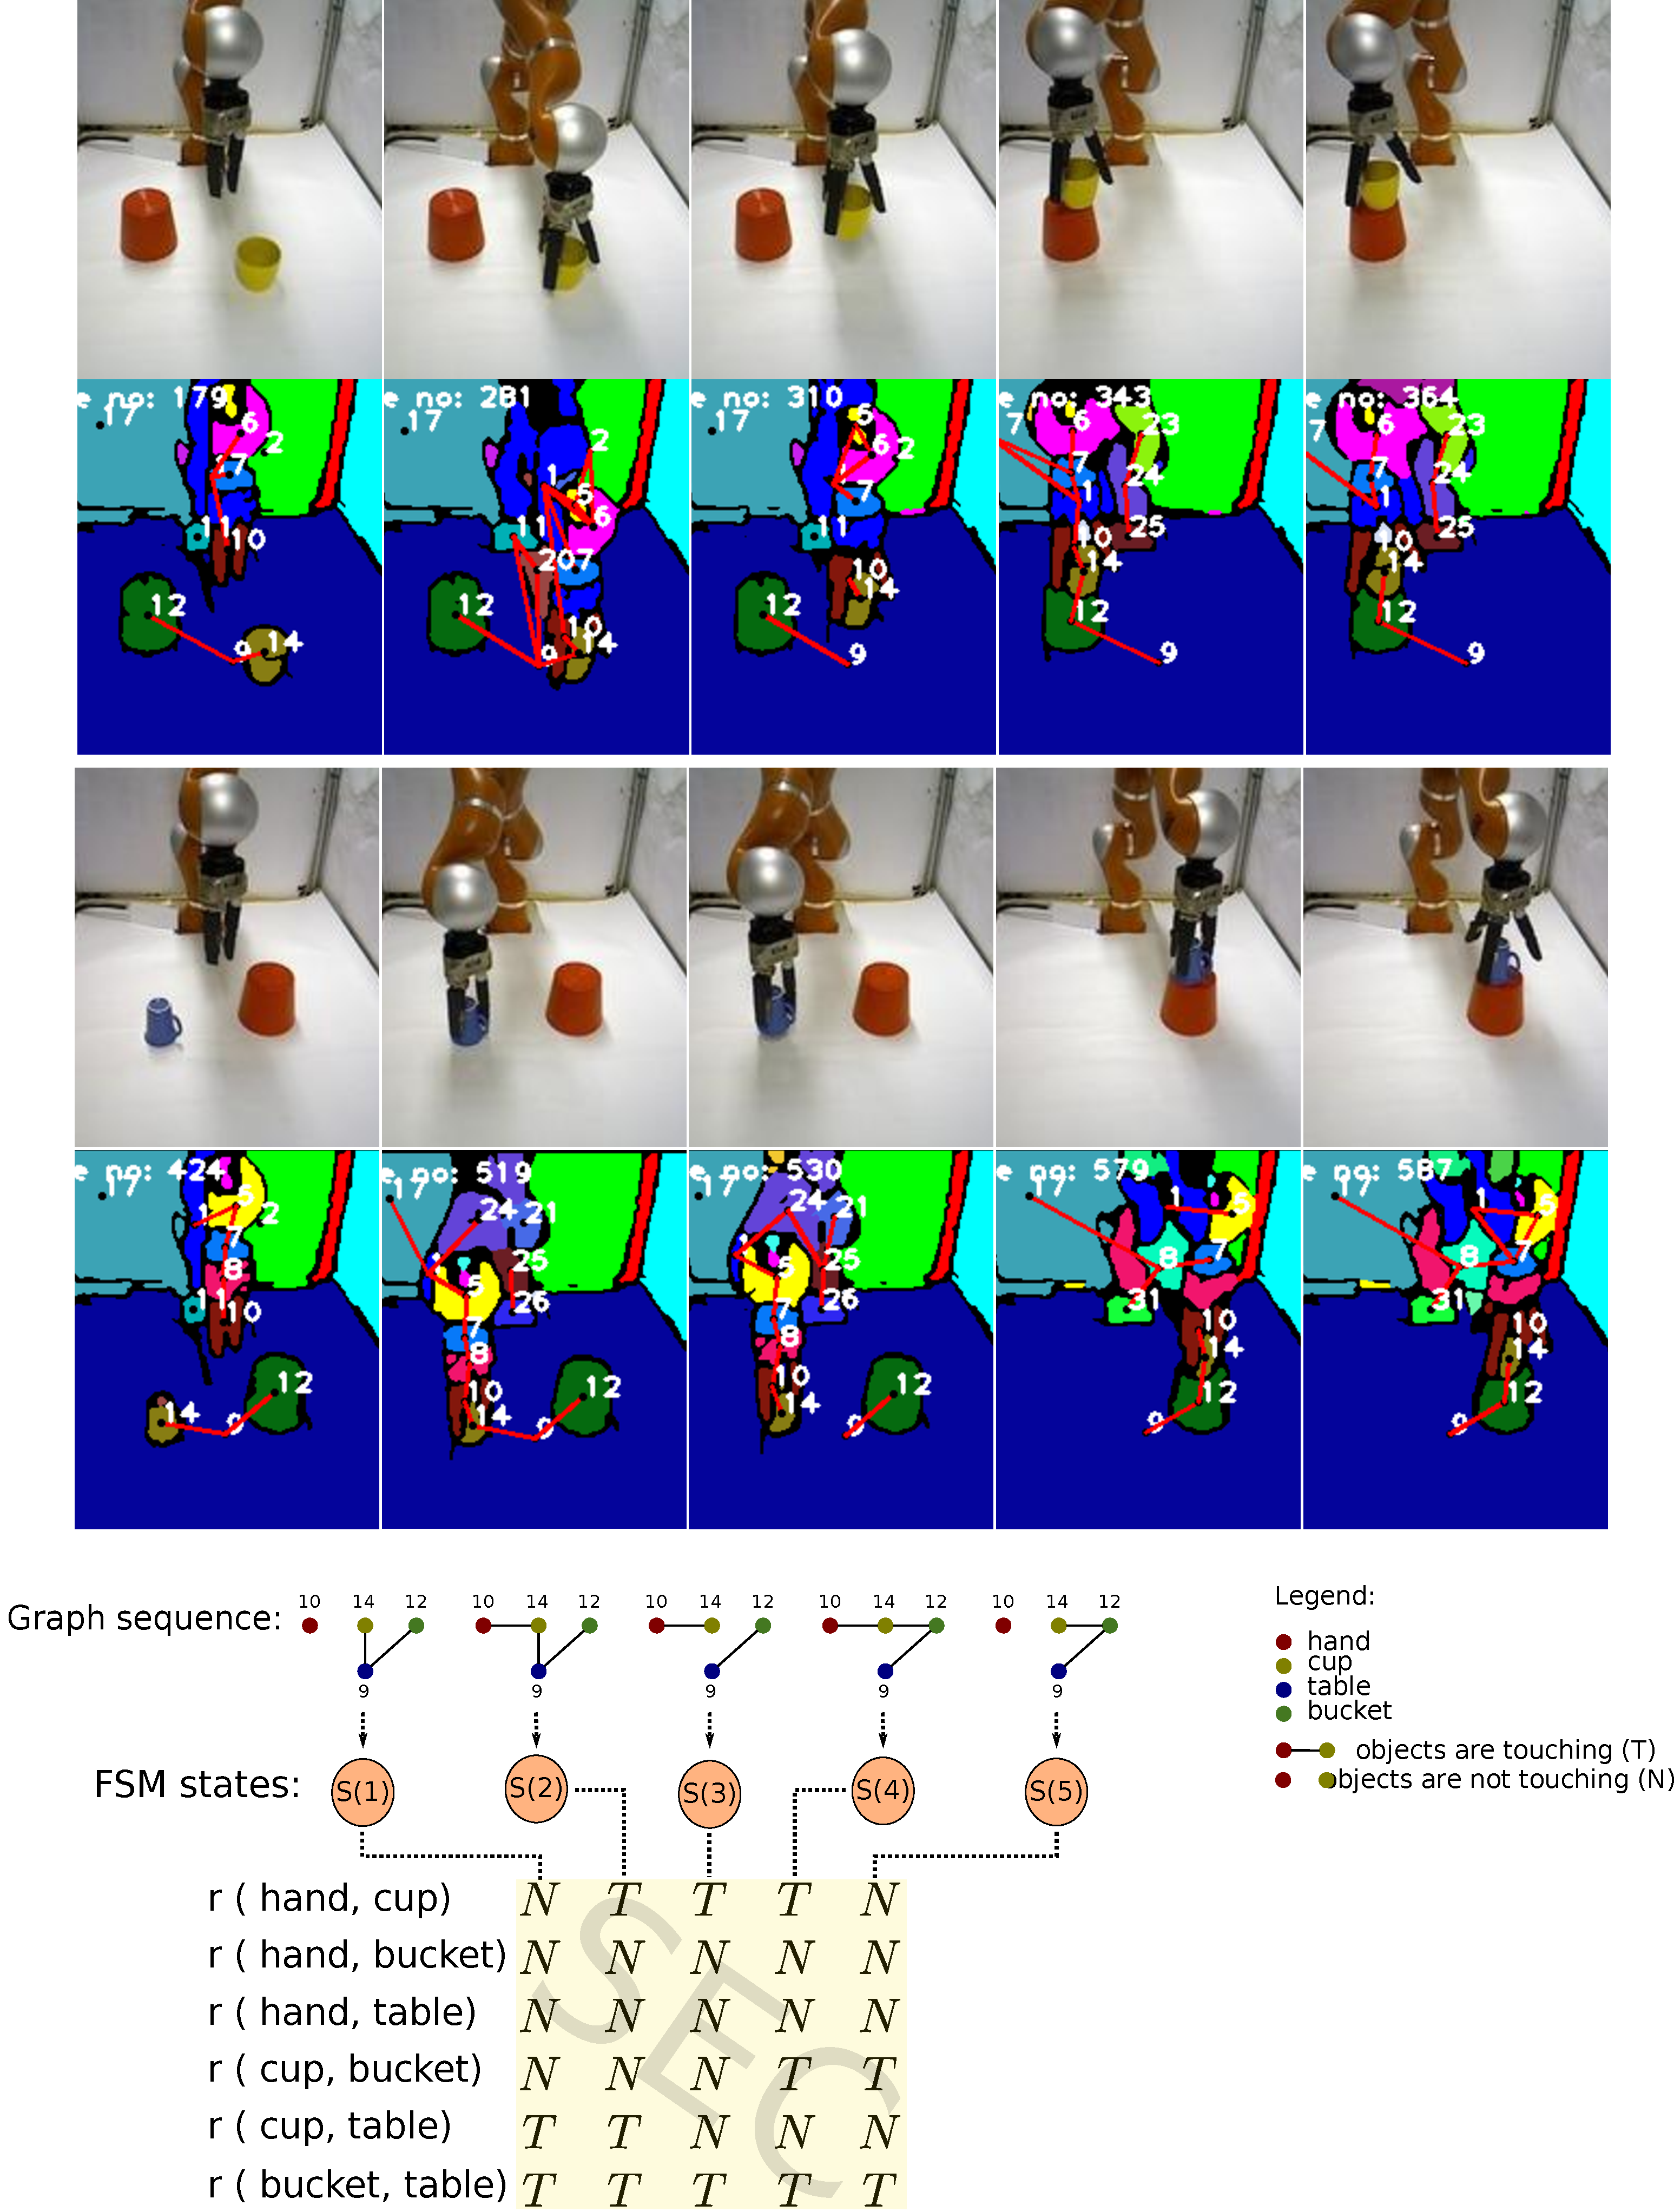
\includegraphics[scale=0.20]{./pdf/result_puton.pdf}
      \caption{ Two instances of the put-on-top action, performed by our method, are shown with different objects and positions. 
The snapshots of the executed actions together with segmented images are shown (top) which indicate the real objects and relations.
The symbolic graph sequence (middle) and the SEC matrix (bottom) remain the same for both version.
}
      \label{fig:result_puton}
\end{figure*}



 








%%%%%%%%%%%%%%%%%%%%%%%%%%%%%%%%%%%%%%%%%%%%%%%%%%%%%%%%%%%%%%%%%%%%%%%%%%%%%%%%%%%%%%%%%%%%%%%%%%%%%%%%%%%%%
\section{Results}
\label{sec:results}

In this section, we will provide experimental results 

\begin{figure*}
      \centering
      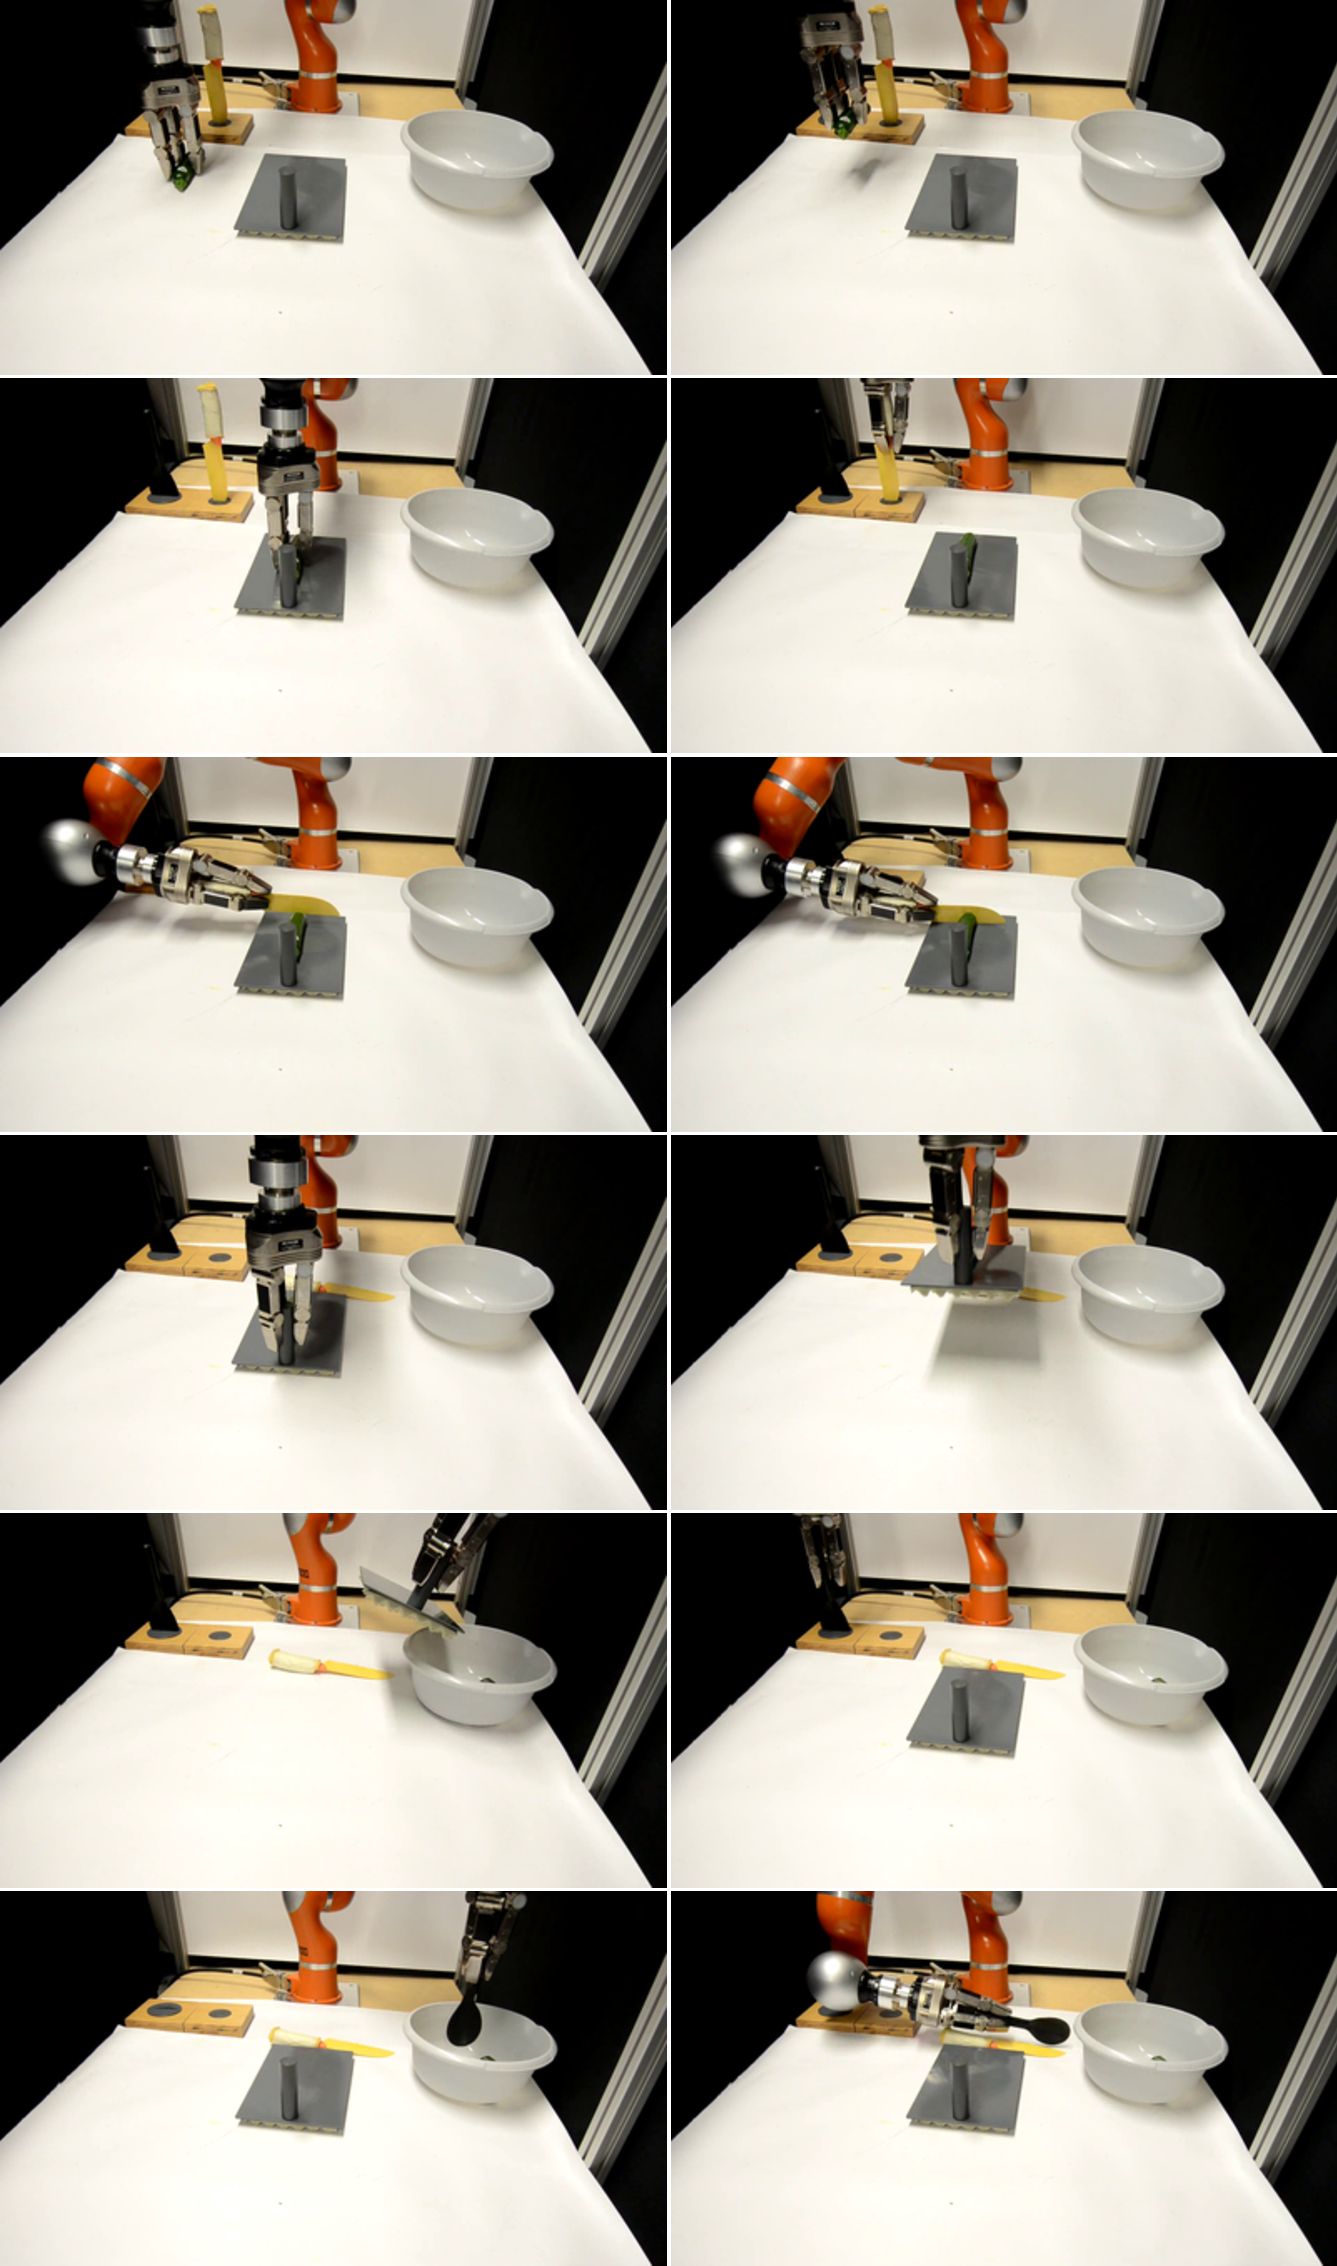
\includegraphics[scale=0.5]{./pdf/scenario_result.pdf}
      \caption{ Two instances of the put-on action, performed by our method, are shown with different objects and positions. 
The snapshots of the executed actions together with segmented images are shown (top) which indicate the real objects and relations.
The symbolic graph sequence (middle) and the SEC matrix (bottom) remain the same for both version.
}
      \label{fig:scenario_result}
\end{figure*}
Several experiments have been conducted in the proposed framework and are available in the library of actions.
The list of the actions are shown in table.\ref{tab:action_list}.


\begin{table*}
\centering
% table caption is above the table
\caption{The list of actions in the library. The last two columns show example objects used in experiments.}
\label{tab:action_list}       % Give a unique label
% For LaTeX tables use
\begin{tabular}{llll}
\hline\noalign{\smallskip}
\# & Action Name & primary obj. & secondary obj. \\
\noalign{\smallskip}\hline\noalign{\smallskip}
1 & pick and place  & cup & - \\
2 & put-on-top & cup, cucumber & bucket, board \\ 
3 & take-down  & cup & bucket \\
4 & put-in  & cup & bucket \\
5 & cut  & knife & zucchini, cucumber, banana \\
6 & unload  & board & zucchini \\
7 & stir  & spoon & milk \\
8 & push  & box & - \\
9 & poke  & box & -\\
\noalign{\smallskip}\hline
\end{tabular}
\end{table*}

The results of the put-on-top example are shown in Fig.\ref{fig:result_puton} for two instances.
For the results of other single actions please see our webpage \url{https://sites.google.com/site/aeinwebpage/actions}.

The actions can be chained to form more complex tasks, like making a salad.
A simple salad making scenario is created by chaining some of the actions in the library.
The scenario is as follows:
\begin{enumerate}
 \item Pick up a zucchini and place it on the cutting board (pick and place action)
 \item Grasp the knife and cut the zucchini (cutting action)
 \item Grasp the board and unload the zucchini pieces into a bowl (unload action)
 \item Grasp a spoon and stir into the bowl (stirring action)
\end{enumerate}

The result is shown in Fig.\ref{fig:scenario_result}.
The video of this scenario is also available in our webpage \url{https://sites.google.com/site/aeinwebpage/actions/videos}.



%%%%%%%%%%%%%%%%%%%%%%%%%%%%%%%%%%%%%%%%%%%%%%%%%%%%%%%%%%%%%%%%%%%%%%%%%%%%%%%%%%%%%%%%%%%%%%%%%%%%%%%%%%%%%
\subsection{Manipulation Observation}
\label{sec:observation}
 
 
 

%%%%%%%%%%%%%%%%%%%%%%%%%%%%%%%%%%%%%%%%%%%%%%%%%%%%%%%%%%%%%%%%%%%%%%%%%%%%%%%%%%%%%%%%%%%%%%%%%%%%%%%%%%%%%
\subsection{Manipulation Action (ManiAc) Dataset}
\label{sec:maniacdataset}
 
%%%%%%%%%%%%%%%%%%%%%%%%%%%%%%%%%%%%%%%%%%%%%%%%%%%%%%%%%%%%%%%%%%%%%%%%%%%%%%%%%%%%%%%%%%%%%%%%%%%%%%%%%%%%%
\section{Discussion}
\label{sec:discussion}

The main contribution of our paper is a novel method for automatic semantic decomposition and recognition of long and complex manipulation sequences.  


%\newpage  %% needed for single columns
%\clearpage  %% needed for two columns
%%%%%%%%%%%%%%%%%%%%%%%%%%%%%%%%%%%%%%%%%%%%%%%%%%%%%%%%%%%%%%%%%%%%%%%%%%%%%%%%%%%%%%%%%%%%%%%%%%%%%%%%%%%%%
\section*{Appendix}
 

%%%%%%%%%%%%%%%%%%%%%%%%%%%%%%%%%%%%%%%%%%%%%%%%%%%%%%%%%%%%%%%%%%%%%%%%%%%%%%%%%%%%%%%%%%%%%%%%%%%%%%%%%%%%%
\begin{acknowledgements}
The research leading to these results has received funding from the European Community’s Seventh Framework Programme FP7/2007-2013 (Programme and Theme: ICT-2011.2.1, Cognitive Systems and Robotics) under grant agreement no. 600578, ACAT. 
\end{acknowledgements}

 


%%%%%%%%%%%%%%%%%%%%%%%%%%%%%%%%%%%%%%%%%%%%%%%%%%%%%%%%%%%%%%%%%%%%%%%%%%%%%%%%%%%%%%%%%%%%%%%%%%%%%%%%%%%%%
 

% BibTeX users please use one of
\bibliographystyle{spbasic}      % basic style, author-year citations
%\bibliographystyle{spmpsci}      % mathematics and physical sciences
%\bibliographystyle{spphys}       % APS-like style for physics
\bibliography{actionlib_journal}   % name your BibTeX data base


% Non-BibTeX users please use
%\begin{thebibliography}{}
%%
%% and use \bibitem to create references. Consult the Instructions
%% for authors for reference list style.
%%
%\bibitem{RefJ}
%% Format for Journal Reference
%Author, Article title, Journal, Volume, page numbers (year)
%% Format for books
%\bibitem{RefB}
%Author, Book title, page numbers. Publisher, place (year)
%% etc
%\end{thebibliography}

\end{document}
% end of file template.tex

